\documentclass[a4paper,11pt]{article}
%\usepackage{minted}
%\usepackage{pygmentize}
\usepackage{graphicx}
\usepackage{float}
\usepackage{subfig}
\usepackage{geometry}
\usepackage{amsmath,amssymb}
\usepackage{amsthm}
\usepackage{bbold}
\usepackage{mathtools}
\usepackage{braket}
\usepackage{booktabs}
\usepackage[table,xcdraw]{xcolor}
\usepackage[utf8]{inputenc}
\usepackage{cite}
\usepackage[english]{babel}
\usepackage{lipsum}
\usepackage{setspace}
<<<<<<< Updated upstream
=======
\usepackage{minted}
>>>>>>> Stashed changes
\usepackage{xcolor}
\newcommand{\R}{\mathbb{R}}
\usepackage{hyperref}
\hypersetup{colorlinks=true,linkcolor=blue}
\geometry{a4paper, top=2.5cm, bottom=2.5cm, left=3cm, right=2.5cm}

\begin{document}
\author{Catalano Giuseppe, Cerrato Nunzia}
\title{Numerical Linear Algebra Homework Project 2:\\Least Squares, Orthogonalization, and the SVD}
\date{}
\maketitle

\section*{Problem 1}
\textbf{(1)} Suppose we are given $m$ pairs of data points, $(x_1,y_1),\dots,(x_m,y_m)$. We want to find a linear combination of prescribed functions $\phi_1, \dots, \phi_n$ whose values at the points $x_i \in [a,b] $, $1\le i \le m$, approximate the values $y_1,\dots, y_m$ as well as possible. More precisely, the problem is to find a function of the form $f(x) = \alpha_1 \phi_1(x) + \dots + \alpha_n \phi_n(x) $ such that 
\begin{equation}
	\sum_{i=1}^{m} \left[ y_i - f(x_i) \right]^2 \le \sum_{i=1}^{m} \left[ y_i - g(x_i) \right]^2\ \ \ \forall g \in \text{Span}(\phi_1,\dots,\phi_n),
\end{equation}
where, usually, $m>n$. It is possible to rephrase the problem as:
\begin{equation}\label{eq: initial definition of the minimization problem}
	f = \arg \min_{f\in \text{Span}(\phi_1,\dots,\phi_n)} \sum_{i=1}^{m} \left[ y_i - f(x_i) \right]^2.
\end{equation}
Now we can define a column vector $\textbf{z} \in \R^n$ such that:
\begin{equation}\label{key}
	[\textbf{z}]_i = \alpha_i
\end{equation}
and a matrix $A$ such that:
\begin{equation}\label{key}
	[A\textbf{z}]_i = f(x_i) = \alpha_1 \phi_1(x_i) + \dots + \alpha_n \phi_n(x_i).
\end{equation}
In this way, the element of the $i-th$ row and $j-th$ column of the matrix $A$ is:
\begin{equation}\label{key}
	[A]_{ij} = a_{ij} = \phi_j(x_i).
\end{equation}
Finally, defining a column vector $\textbf{b} \in \R^n$ such that:
\begin{equation}\label{key}
	[\textbf{b}]_i = y_i
\end{equation}
we can rewrite the \eqref{eq: initial definition of the minimization problem} as follows:
\begin{equation}\label{key}
	\tilde{\textbf{z}} = \arg \min_{\textbf{z}\in \R^n} \lVert \textbf{b} - A \textbf{z} \rVert_2^2 =  \arg \min_{\textbf{z}\in \R^n} \lVert \textbf{b} - A \textbf{z} \rVert_2,
\end{equation}
where the function $f$ can be built from $\tilde{\textbf{z}}$.

\noindent \textbf{(2)} Now we suppose to take $\phi_k = x^{k-1}$, $1 \le k \le n$. Under this assumption, the matrix $A$ takes the form:
\begin{equation}\label{key}
	A = \begin{bmatrix}
		x_1^0 & \cdots & x_1^{n-1}  \\
		\vdots & \ddots & \vdots \\
		x_m^0 & \cdots  & x_m^{n-1}
	\end{bmatrix}.
\end{equation}
We want to prove that, assuming that $x_i\neq x_j$ for $i \neq j$, $A$ has full rank: $\text{rank}(A) = n$.\\
Proof: Proving that $\text{rank}(A) = n$ is equivalent to prove that $\dim(\ker(A)) = 0$, that means that $\nexists \textbf{v} \in \R^n \text{ s.t. } \textbf{v} \in \ker(A)$. We want to prove this statement by contraddiction, therefore, we look for a vector $\textbf{v} \in \R^n$, with $\textbf{v} \neq \underline{0}$, such that $A\textbf{v}=\underline{0}$, that means:
\begin{equation}\label{key}
	\left\lbrace 
	\begin{split}
		&  v_1 x_1^0 + \dots + v_n x_1^{n-1} = 0\\
		& \vdots  \\
		&  v_1 x_m^0 + \dots + v_n x_m^{n-1} = 0 
	\end{split} \right.  .
\end{equation}
Defining the polynomial 
\begin{equation}\label{key}
	p^{(n-1)}_{\textbf{v}}(x) = \sum_{i=1}^{n} v_i x^{i-1}
\end{equation}
we can observe that, for any choice of $\textbf{v} \neq \underline{0}$, $p^{(n-1)}_{\textbf{v}}(x)$ admits at most $n-1$ different roots, therefore $\nexists \textbf{v} \neq \underline{0}$ such that $A\textbf{v}=\underline{0}$. This concludes the proof. \qedsymbol

\noindent \textbf{(3)} Consider the problem of finding the best fit with a quadratic function $f(x) = \alpha_1 + \alpha_2 x + \alpha_3 x^2$ for the following data:\\
\begin{center}	
\begin{tabular}{c|c|c|c|c|c|c|c|c|c}
	$x_i$& 8 & 10 & 12 & 16 & 20 & 30 & 40 & 60 & 100 \\
	\hline
	$y_i$& 0.88 & 1.22 & 1.64 & 2.72 & 3.96 & 7.66 & 11.96 & 21.56 & 43.16 \\
\end{tabular}.
\end{center}
In the following we report the code that solves the normal equations:
\begin{equation}\label{key}
	A^T A \textbf{v} = A^T \textbf{b}
\end{equation}
using the Cholesky factorization algorithm and then compares the result with the one found using the QR factorization of the matrix $A$.

\noindent *** INSERIRE CODICE ***

\noindent Using the previous functions we have computed the solution to the minimization problem, obtaining the following results:\\
\begin{tabular}{cc}
	Cholesky:  &$x = [-1.91914925269909,\   0.278213536291725,\ 0.001739400875055]$\\
	QR factorization:&$x = [-1.91914925269904,\  0.278213536291722,\ 0.001739400875055]$ \\
\end{tabular}.

\noindent From these results we can observe that, for this problem, both the algorithms perform in a similar way. In fact, the results differ at most in the 15th digit. In figure \ref{fig: fit and data Cholesky QR} we show the input data and the solutions to the least square problem.

\begin{figure}[t]
	\centering
	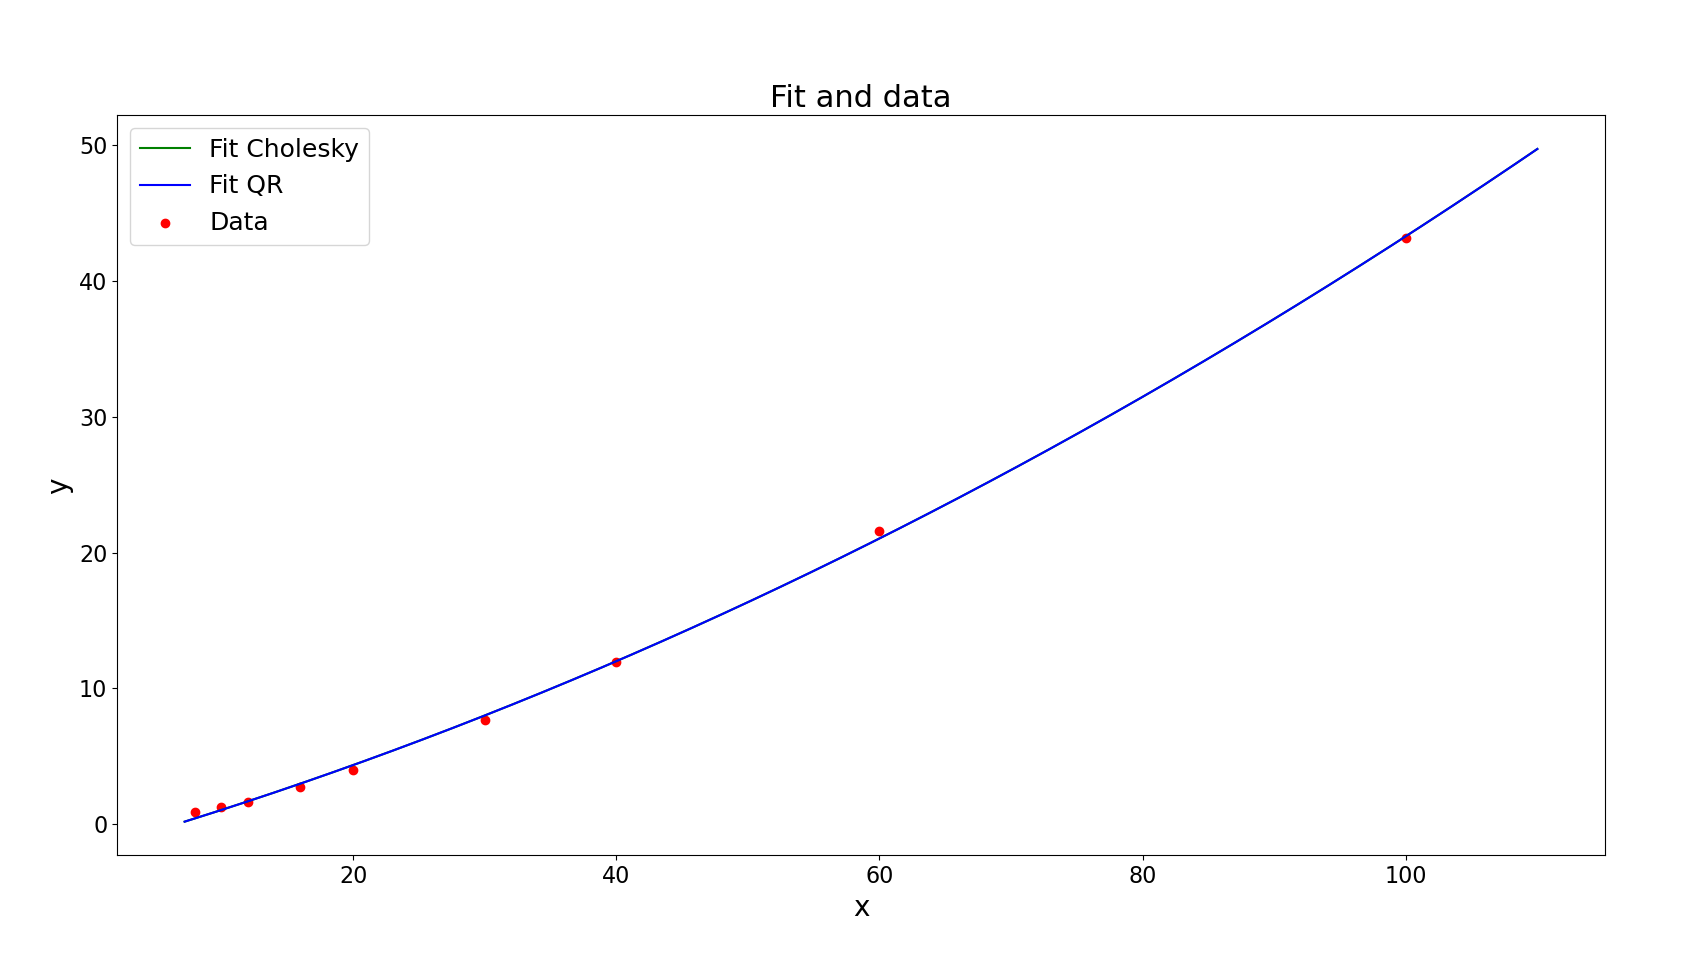
\includegraphics[width=1.1\linewidth]{../Project_2_latex/Plot/Fit_and_data.png}
	\caption{}
	\label{fig: fit and data Cholesky QR}
\end{figure}



\noindent \textbf{(4)} The following code computes the residual $\textbf{r} = \textbf{d} - C\hat{\textbf{x}}$ where $\hat{\textbf{x}} =  \left[  - 1.919,\  0.2782,\  0.001739\right] $ is the approximate solution of the least squares problem.

\noindent ***INSERIRE CODICE***\\

\noindent The results that we obtain are:\\
\begin{tabular}{cc}
 	Residual: &$\textbf{r}  = [ 0.009503999999993,\  0.716895999999906,\ 62.090847999905236]$\\
 	Norm 2 of the residual: &$\lVert  \textbf{r}  \rVert_2 = 62.09498720144942$\\
\end{tabular}.\\
The value of the residual may seem strange, in fact, if we compute the relative error we find:
\begin{equation}\label{key}
	\frac{\lVert  \textbf{x} - \hat{\textbf{x}} \rVert_2 }{\lVert  \textbf{x} \rVert_2 }  = 7.728184292875672\text{e-05}.
\end{equation}

\noindent However, we can observe that, from the relation
\begin{equation}\label{key}
	\frac{1}{k_2(C)} \frac{\lVert  \textbf{r}  \rVert_2 }{\lVert  \textbf{d}  \rVert_2 } \le \frac{\lVert  \textbf{x} - \hat{\textbf{x}} \rVert_2 }{\lVert  \textbf{x} \rVert_2 } \le k_2(C) \frac{\lVert  \textbf{r}  \rVert_2 }{\lVert  \textbf{d}  \rVert_2 }
\end{equation}
we can obtain the following relation for $\textbf{r} $:
\begin{equation}\label{key}
	\frac{\lVert  \textbf{d}  \rVert_2}{k_2(C)} \frac{\lVert  \textbf{x} - \hat{\textbf{x}} \rVert_2 }{\lVert  \textbf{x} \rVert_2 }\le \lVert  \textbf{r}  \rVert_2 \le k_2(C) \lVert  \textbf{d}  \rVert_2 \frac{\lVert  \textbf{x} - \hat{\textbf{x}} \rVert_2 }{\lVert  \textbf{x} \rVert_2 }.
\end{equation}

\noindent With the following python code we have computed the bounds to the residual.
*** INSERIRE CODICE***\\

\noindent From the output of the previous code we know that:
\begin{equation}\label{key}
	5 \times 10^{-7} \lessapprox \lVert  \textbf{r}  \rVert_2 \lessapprox 3 \times 10^9
\end{equation}
this big range is due to the value of $k_2(C)  \simeq 8 \times 10^7$ that suggests us that we should not use the residual to measure the accuracy of the solution when the problem is ill-conditioned as in this case. 

\section*{Problem 2}
\textbf{(1)} Let $A \in \R^{m\times n}$, with $\text{rank}(A) = n$, let {A = QR} be the (full) QR factorization of $A$, with $Q \in \R^{m\times m} $ orthogonal and $R \in \R^{m\times n}$ upper trapezoidal. Also, let $A = Q_1 R_1$ be the reduced QR factorization of $A$ with $Q_1 \in \R^{m\times n}$ having orthonormal columns and $R_1 \in \R^{m\times m}$ upper triangular. Show that $R_1$ is nonsingular, and that the columns $\textbf{q}_1 . . . , \textbf{q}_n$ of $Q_1$ form an orthonormal basis for $\text{Ran}(A)$, the column space of $A$. Also, find an orthonormal basis for $\text{Null}(A^T)$, the null space of $A^T$ .\\
We start showing that $R_1$ is nonsingular. Since $A$ has full rank, we know that:
\begin{equation}\label{key}
	A \textbf{x} = \textbf{0} \Leftrightarrow \textbf{x} = \textbf{0}
\end{equation}
and multiplying both sides for $Q_1^T$ knowing that $Q_1^T Q_1 = \mathcal{I}_n$ we obtain
\begin{equation}\label{key}
	R_1 \textbf{x} = \textbf{0} \Leftrightarrow \textbf{x} = \textbf{0},
\end{equation}
that concludes the proof.\\
Now we want to show that the columns $\textbf{q}_1 . . . , \textbf{q}_n$ of $Q_1$ form an orthonormal basis for $\text{Ran}(A)$. We start observing that 
\begin{equation}\label{key}
	\forall \textbf{y} \in \text{Ran}(A) \exists \textbf{x} \in \R^n : \textbf{y} = A \textbf{x} = Q_1R_1\textbf{x}
\end{equation}
and we know this from the definition of range of a matrix. In a similar way, knowing that $R_1$ is nonsingular and therefore is a bijective map from $\R^n$ to $\R^n$, we can put $\textbf{x}' = R_i \textbf{x}$ and say that:
\begin{equation}\label{key}
	\forall \textbf{y} \in \text{Ran}(A) \exists \textbf{x} \in \R^n : \textbf{y} = A \textbf{x} = Q_1\textbf{x}',
\end{equation}
that means that $\text{Ran}(A) = \text{Ran}(Q_1) = \text{Span}\{\textbf{q}_1,\dots,\textbf{q}_n\}$.\\
Now we want to find an orthonormal basis for $\text{Null}(A^T)$. Knowing that $\text{Null}(A^T) = (\text{Ran}(A))^\perp$ we can, immediately, find the solution. In fact:
\begin{equation}\label{key}
	(\text{Ran}(A))^\perp = \text{Span}\{\textbf{q}_1,\dots,\textbf{q}_n\}^\perp = \text{Span}\{\textbf{q}_{n+1}\dots,\textbf{q}_m\}.
\end{equation}
This concludes the proof. \qed\\

\noindent \textbf{(2)} Given tha full rank matrix
\begin{equation}\label{key}
	A = \begin{bmatrix}
		1.07 & 1.10  \\
		1.07 & 1.11  \\
		1.07 & 1.15 
	\end{bmatrix},
\end{equation}
compute $A^T A$ in $\beta = 10$, $t=3$ digit arithmetic and verify if $A^T A$ is positive definite.\\
We performed the prescribed calculation using the rounding function
\begin{equation}\label{key}
	\text{fl}(x) = \arg \min_{y\in \mathbb{F}} |y-x|
\end{equation}
where $\mathbb{F} = \{\pm(0.d_1d_2d_3)\times 10^p : d_i \in {0,\dots,9},\ -2046\le p \le 2046\}$ and, when there is ambiguity, we approximate always away from $0$. Moreover, the rounding function has been applied at each step of the calculation, meaning that, if we consider $\textbf{v}, \textbf{u} \in \R^n$
\begin{equation}\label{key}
	\textbf{v}^T \textbf{u} = \text{fl} \left( \sum_{i=1}^{n}\text{fl} (v_i u_i)\right) .
\end{equation}
The result of the calculation is the following:
\begin{equation}\label{key}
	A^T A =  \begin{bmatrix}
		3.42 & 3.6  \\
		3.6 & 3.76  \\
	\end{bmatrix}.
\end{equation}
The last matrix is indefinite, in fact $\text{Det}(A^T A) = 3.42 \times 3.76 - 3.6^2 = 12.8592 -  12.96 < 0$.\\

\noindent \textbf{(3)} Compute the QR factorization of the matrix
\begin{equation}\label{key}
	A = \begin{bmatrix}
		1.07 & 1.10  \\
		1.07 & 1.11  \\
		1.07 & 1.15 
	\end{bmatrix} = [\textbf{a}_1\ \textbf{a}_2]
\end{equation}
in 3 digit arithmetic, i.e. with $\beta = 10$, $t=3$. The $\text{fl}(x)$ function has been applied at each step, as in the previous exercise.\\
We want to compute $H_1 A$:
\begin{equation}\label{key}
	H_1 A = \begin{bmatrix}
				r_{11} & \textbf{r}_1^T  \\
		\textbf{0} & A_1  \\
	\end{bmatrix}.
\end{equation} 
\begin{equation}\label{key}
	r_{11} = -\text{sgn}(a_{11})\lVert \textbf{a}_1\rVert_2 = \lVert \textbf{a}_1\rVert_2 = \sqrt{1.14 \times 3 }= \sqrt{3.42} = -1.85
\end{equation}

\begin{equation}\label{key}
	\hat{\textbf{u}}_1  = \textbf{a}_1 + r_{11} \textbf{e}_1 = \begin{pmatrix}
		1.07\\
		1.07\\
		1.07
	\end{pmatrix} + 1.85 \begin{pmatrix}
	1\\
	0\\
	0
\end{pmatrix} = \begin{pmatrix}
2.92\\
1.07\\
1.07
\end{pmatrix}
\end{equation}

\begin{equation}\label{key}
	\lVert \hat{\textbf{u}} \rVert_2 = \sqrt{8.53 + 1.14 + 1.14} = \sqrt{10.81} = 3.29
\end{equation}

\begin{equation}\label{key}
		\textbf{u}_1 = 	\hat{\textbf{u}}_1/\lVert \hat{\textbf{u}} \rVert_2  =  \begin{pmatrix}
			0.888\\
			0.325\\
			0.325
		\end{pmatrix} 
\end{equation}

\begin{equation}\label{key}
	\begin{split}
		H_1 \textbf{a}_2 &= \textbf{a}_2 - 2 (\textbf{u}_1^T\textbf{a}_2) \textbf{u}_1  \\
		&= \begin{pmatrix}
			1.10\\
			1.11\\
			1.15
		\end{pmatrix} - 2(0.977 + 0374 + 0.374) \begin{pmatrix}
		0.888\\
		0.325\\
		0.325
	\end{pmatrix} \\
	&= \begin{pmatrix}
		1.10\\
		1.11\\
		1.15
	\end{pmatrix} - 3.42 \begin{pmatrix}
		0.888\\
		0.325\\
		0.325
	\end{pmatrix} = \begin{pmatrix}
	-1.94\\
	0\\
	0.04
\end{pmatrix}
	\end{split} .
\end{equation}
Therefore we have:
\begin{equation}\label{key}
	H_1 A = \begin{pmatrix}
		-1.85& -1.94 \\
		0& 0  \\
		0& 0.04
	\end{pmatrix}. 
\end{equation}
Now we iterate the same procedure on $A_1$, with
\begin{equation}\label{key}
	A_1 = [\textbf{a}_2^{(1)}] = \begin{pmatrix}
		0\\
		0.04
	\end{pmatrix}.
\end{equation}


\begin{equation}\label{key}
	\hat{\textbf{u}}_2^{(1)} = \textbf{a}_2^{(1)} + \text{sgn}(a_{12}^{(1)}) \lVert \textbf{a}_2^{(1)} \rVert_2\textbf{e}_2^{(1)} = \begin{pmatrix}
		0\\
		0.04
	\end{pmatrix}+ \text{sgn}(0) 0.04 \begin{pmatrix}
		1\\
		0
	\end{pmatrix} = \begin{pmatrix}
		0.04\\
		0.04
	\end{pmatrix}
\end{equation}


\begin{equation}\label{key}
	\textbf{u}_2^{(1)} = \hat{\textbf{u}}_2^{(1)}/ \lVert \hat{\textbf{u}}_2 ^{(1)}\rVert_2 = \begin{pmatrix}
		0.707\\
		0.707
	\end{pmatrix}.
\end{equation}

\noindent The complete vector $\textbf{u}_2$ will be:
\begin{equation}\label{key}
	\textbf{u}_2 = \begin{pmatrix}
		0\\
		0.707\\
		0.707
	\end{pmatrix}
\end{equation}
and the element $r_{22}$ willl be
\begin{equation}\label{key}
	r_{22} = - \text{sgn}(a_{12}^{(1)}) \lVert \textbf{a}_2^{(1)} \rVert_2 = -0.04
\end{equation}
so that, finally, we have
\begin{equation}\label{key}
	H_2 H_1 A = R = \begin{pmatrix}
		-1.85& -1.94 \\
		0& -0.04  \\
		0& 0
	\end{pmatrix}.
\end{equation}
We can observe that the matrix $R$ is full rank, therefore it is possible to use the QR factorization to solve the least square problem. It is important to stress that, as $A^T A$ is indefinite in $3$ digit precision, using Cholesky is not possible.\\
Now we want to compute $Q=[\textbf{q}_1,\textbf{q}_2,\textbf{q}_3]$ and, in order to do it, we use the following relations:
\begin{equation}\label{key}
	\begin{split}
		&\textbf{q}_1 = H_1 H_2 \textbf{e}_1 = \textbf{e}_1 - 2 (\textbf{u}_1^T \textbf{e}_1) \textbf{u}_1\\
		&  \textbf{q}_2 = H_1 H_2 \textbf{e}_2 = H_1 (\textbf{e}_2 - 2 (\textbf{u}_2^T \textbf{e}_2) \textbf{u}_2)  \\
		&=  \textbf{e}_2 - 2 (\textbf{u}_2^T \textbf{e}_2) \textbf{u}_2 -  2 (\textbf{u}_1^T \textbf{e}_2) \textbf{u}_1  + 4 (\textbf{u}_2^T \textbf{e}_2)(\textbf{u}_1^T \textbf{u}_2)\textbf{u}_1\\
		&  \textbf{q}_3 = H_1 H_2 \textbf{e}_3 = H_1 (\textbf{e}_3 - 2 (\textbf{u}_2^T \textbf{e}_3) \textbf{u}_2)  \\
		&=  \textbf{e}_3 - 2 (\textbf{u}_2^T \textbf{e}_3) \textbf{u}_2 -  2 (\textbf{u}_1^T \textbf{e}_3) \textbf{u}_1  + 4 (\textbf{u}_2^T \textbf{e}_3)(\textbf{u}_1^T \textbf{u}_2)\textbf{u}_1
	\end{split}.
\end{equation}
Using these relations, we found the approximated matrix $Q$, that is:
\begin{equation}\label{key}
	Q = \begin{bmatrix}
		-0.578& 0.572 & 0.572 \\
		-0.578& 0.212 & -0.788 \\
		-0.578& -0.788 & 0.212
	\end{bmatrix}.
\end{equation}
Finally, we can verify that, multiplying $Q$ and $R$ and approximating as before, we recover the original matrix $A$. It is important to point out that the columns of $Q$ are not perfectly orthonormal.\\

\noindent \textbf{(4)} Let $A \in \R^{m\times n}$, with $\text{rank}(A) = n$, and let $\textbf{b} \in \R^m$. Let $A = Q_1R_1$ be a reduced QR decomposition of $A$, where $Q_1 \in \R^{m\times n}$ has orthonormal columns and $R_1 \in \R^{n\times n}$ is upper triangular and nonsingular. Show that a reduced QR factorization of the augmented matrix $A_+ = [ A\ \textbf{b} ]$ is given by:
\begin{equation}\label{key}
	A_+=[Q_1\  \textbf{q}_{n+1}] \begin{bmatrix}
		R_1& \textbf{z}  \\
		\textbf{0}^T& \rho 
	\end{bmatrix}
\end{equation}
where $\textbf{z} = Q_1^T\textbf{b}$. Also, show that $|\rho| = \lVert \textbf{b} - A \textbf{x}^*\rVert_2$ where $\textbf{x}^*$ is the solution to the least squares problem $\lVert \textbf{b} - A \textbf{x}\rVert_2= \text{min} $.\\
We start recalling that any matrix has a QR factorization, therefore the matrix $A_+$ must have it. In particular we know that $A_+ = Q_+ R_+$, where $Q_+$ has orthonormal columns and $R_+$ is upper triangular. In order to find the value of $\textbf{z}$ and $\rho$, we compute the product $Q_+ R_+$ and impose that it is equal to $A_+$:
\begin{equation}\label{key}
	[Q_1\  \textbf{q}_{n+1}] \begin{bmatrix}
		R_1& \textbf{z}  \\
		\textbf{0}^T& \rho 
	\end{bmatrix} = [Q_1 R_1\ Q_1\textbf{z} + \rho \textbf{q}_{n+1}] = [A\ \textbf{b}],
\end{equation}
therefore we must have 
\begin{equation}\label{key}
	\textbf{b} = Q_1 \textbf{z} + \rho \textbf{q}_{n+1}.
\end{equation}
Multiplying both members of the last equation for $Q_1^T$ we find that:
\begin{equation}\label{key}
	Q_1^T \textbf{b} = Q_1^T Q_1 \textbf{z} +  \rho Q_1^T \textbf{q}_{n+1} = \textbf{z}
\end{equation}
where we used that the columns of $Q_1$ are orthonormal and $\textbf{q}_{n+1}$ is orthogonal to all the columns of $Q_1$.\\
Now we consider the complete QR factorization of $A_+$:
\begin{equation}
	A_+ =QR= [Q_1\ Q_2] \left[ \begin{tabular}{c}
		\begin{tabular}{cc}
			$R_1$& $\textbf{z}$ \\
			$\textbf{0}^T$& $\rho$ \\
		\end{tabular}\\
	\hline
		$\textbf{0}$
	\end{tabular}\right] = [Q_1 R_1\ \ Q_1 \textbf{z} + Q_2(\rho,0,\dots,0)^T  ]
\end{equation}
obtaining the relation
\begin{equation}\label{key}
	\textbf{b} = Q_1 \textbf{z} + Q_2(\rho,0,\dots,0)^T
\end{equation}
and, therefore, multiplying both sides for $Q_2^T$:
\begin{equation}\label{key}
	Q_2^T \textbf{b} = \rho (1,0,\dots,0)^T.
\end{equation}

\noindent Now we define the residual $\textbf{r}$ as
\begin{equation}\label{key}
	\textbf{r} = \textbf{b} - A \textbf{x}^*
\end{equation}
where $ \textbf{x}^*$ is the solution to the least square problem, and compute:
\begin{equation}\label{key}
	\lVert \textbf{r} \rVert_2^2 = \lVert Q^T \textbf{r} \rVert_2^2 = \lVert \begin{bmatrix}
		Q_1^T \textbf{b}\\
		Q_2^T \textbf{b}
	\end{bmatrix} -\begin{bmatrix}
		Q_1^T A \textbf{x}^*\\
		Q_2^T A \textbf{x}^*
	\end{bmatrix} \rVert_2^2 = \lVert Q_1^T \textbf{b} - R_1 \textbf{x}^* \rVert_2^2 + \lVert Q_2^T \textbf{b} \rVert_2^2
\end{equation}
where we used the invariance of the 2-norm with respect to unitary transformations. Knowing that $\textbf{x}^* = R_1^{-1} Q_1^T \textbf{b}$ we obtain:
\begin{equation}\label{key}
	\lVert \textbf{r} \rVert_2 = \lVert Q_2^T \textbf{b} \rVert_2 = \lVert \rho (1,0,\dots,0)^T \rVert_2 = |\rho|
\end{equation}
that concludes the proof. \qed

\section*{Problem 3}

\noindent \textbf{(1)} Let $A \in \R^{m\times n}$, with $\text{rank}(A) = n$. The singular value decomposition of $A$ can be written as $A = U \Sigma V^T$ or, equivalently, as $A = \sum_{i=1}^n \sigma_i \textbf{u}_i \textbf{v}_i^T$, where $\sigma_1 \ge \sigma_2 \ge \dots \ge \sigma_n$ represent the singular values of $A$, while $\{\textbf{u}_{i}\}_{i=1,\dots,n}$ and $\{\textbf{v}_{i}\}_{i=1,\dots,n}$ are, respectively, left and right singular vectors of $A$.\\

\noindent Express the singular values and singular vectors of the following matrices in terms of those of $A$.\\

\noindent \textbf{(a)} {$(A^{T}A)^{-1}$}
\[(A^{T}A)^{-1} = (V^{T})^{-1}\Sigma^{-2}V^{-1}=V\Sigma^{-2}V^{T}\]
In order to obtain this expression we used that $U^{T}U=\mathbb{1}$ and that $V^{-1}=V^{T}$, since $U$ and $V$ are orthogonal. We can conclude that both left and right singular vectors of $(A^{T}A)^{-1}$ are equal to the right singular vectors of $A$, while singular values of the former matrix are equal to those of $A$ raised to the $-2$ power. Note that, since singular values of $A$ are in increasing order and in this expression they are raised to a negative power, they must appear in reverse order.\\

%\begin{itemize}
%	\item Both left and right singular vectors of $(A^{T}A)^{-1}$ are equal to the right singular vectors of $A$;
%	\item Singular values of $(A^{T}A)^{-1}$ are equal to singular values of $A$ raised to the $-2$ power.
%\end{itemize}

\noindent \textbf{(b)} $(A^{T}A)^{-1}A^{T}$
\[(A^{T}A)^{-1}A^{T} = V\Sigma^{-2}V^{T}V\Sigma U^{T}=V\Sigma^{-1}U^{T}\]
Analogously to the previous case, we know that $V^{T}V=\mathbb{1}$. Here we see that left singular vectors of $(A^{T}A)^{-1}A^{T}$ are equal to the right singular vectors of $A$, right singular vectors of $(A^{T}A)^{-1}A^{T}$ are equal to the left singular vectors of $A$, while singular values of this matrix are equal to the inverse of singular values of $A$.\\

%\begin{itemize}
%	\item Left singular vectors of $(A^{T}A)^{-1}A^{T}$ are equal to the right singular vectors of $A$;
%	\item Right singular vectors of $(A^{T}A)^{-1}$ are equal to the left singular vectors of $A$;
%	\item Singular values of $(A^{T}A)^{-1}$ are equal to the inverse of singular values of $A$.
%\end{itemize}

\noindent \textbf{(c)} $A(A^{T}A)^{-1}$
\[A(A^{T}A)^{-1} = U\Sigma V^{T}V\Sigma^{-2}V^{-T}=U\Sigma^{-1}V^{T}\]
Note that this result can also be obtained from the previous case, by noting that $A(A^{T}A)^{-1}=((A^{T}A)^{-1}A^{T})^{T}$. We can see that left and right singular vectors of $(A^{T}A)^{-1}$ coincide with that of $A$, while singular values of this matrix are equal to the inverse of singular values of $A$.\\
%\begin{itemize}
%	\item Left and right singular vectors of $(A^{T}A)^{-1}$ coincide with that of $A$;
%	\item Singular values of $(A^{T}A)^{-1}$ are equal to the inverse of singular values of $A$.
%\end{itemize}

\noindent \textbf{(d)} $A(A^{T}A)^{-1}A^{T}$
\[A(A^{T}A)^{-1}A^{T} = U\Sigma^{-1}V^{T}V\Sigma U^{T}= U U^{T} \]
In this case, both left and right singular vectors of $A(A^{T}A)^{-1}A^{T}$ are equal to left singular vectors of $A$, while singular values of this matrix are all equal to $1$.\\


\noindent \textbf{(2)} Given the following matrix:
\begin{equation}
	A = \begin{bmatrix}
		1 & 2 \\
		0 & 2
	\end{bmatrix},
\end{equation}
its singular values can be computed by considering the square root of the eigenvalues of the matrix $A^{T}A$, which has the form:
\begin{equation}
	A^{T}A = \begin{bmatrix}
		1 & 2 \\
		2 & 8
	\end{bmatrix}.
\end{equation}
Hence, by imposing that $p(\lambda)=\det(A^{T}A -\lambda\mathbb{1})=0$, we find the two eigenvalues of $A^{T}A$ and, therefore, the two singular values of $A$, which are:
\begin{equation}
	\sigma_{1,2}=\sqrt{\frac{9 \pm \sqrt{65}}{2}}.
\end{equation}
Finally, knowing that the spectral condition number is defined as $k_{2}(A) = \frac{\sigma_{\max}}{\sigma_{\min}}$, we can find the condition number of $A$:
\begin{equation}
	k_{2}(A) = \sqrt{\frac{9+\sqrt{65}}{9-\sqrt{65}}} \simeq 4.26.
\end{equation}
We want now to see how the unit ball is modified by the transformation described by the matrix $A$. In other words, we want to see what is the image of a vector $\textbf{x}=(\cos(\theta),\sin(\theta))$, parametrizing the unit ball on a plane, when considering the linear transformation $\textbf{y}=A\textbf{x}$. The vector $\textbf{y}$ under the transformation $A$ assumes the form:
\[\textbf{y}=(\cos(\theta) + 2\sin(\theta), 2\sin(\theta)) \quad \theta \in \left[0,2\pi\right).\]
Graphically, we have:
\begin{figure}[H]
	\centering
	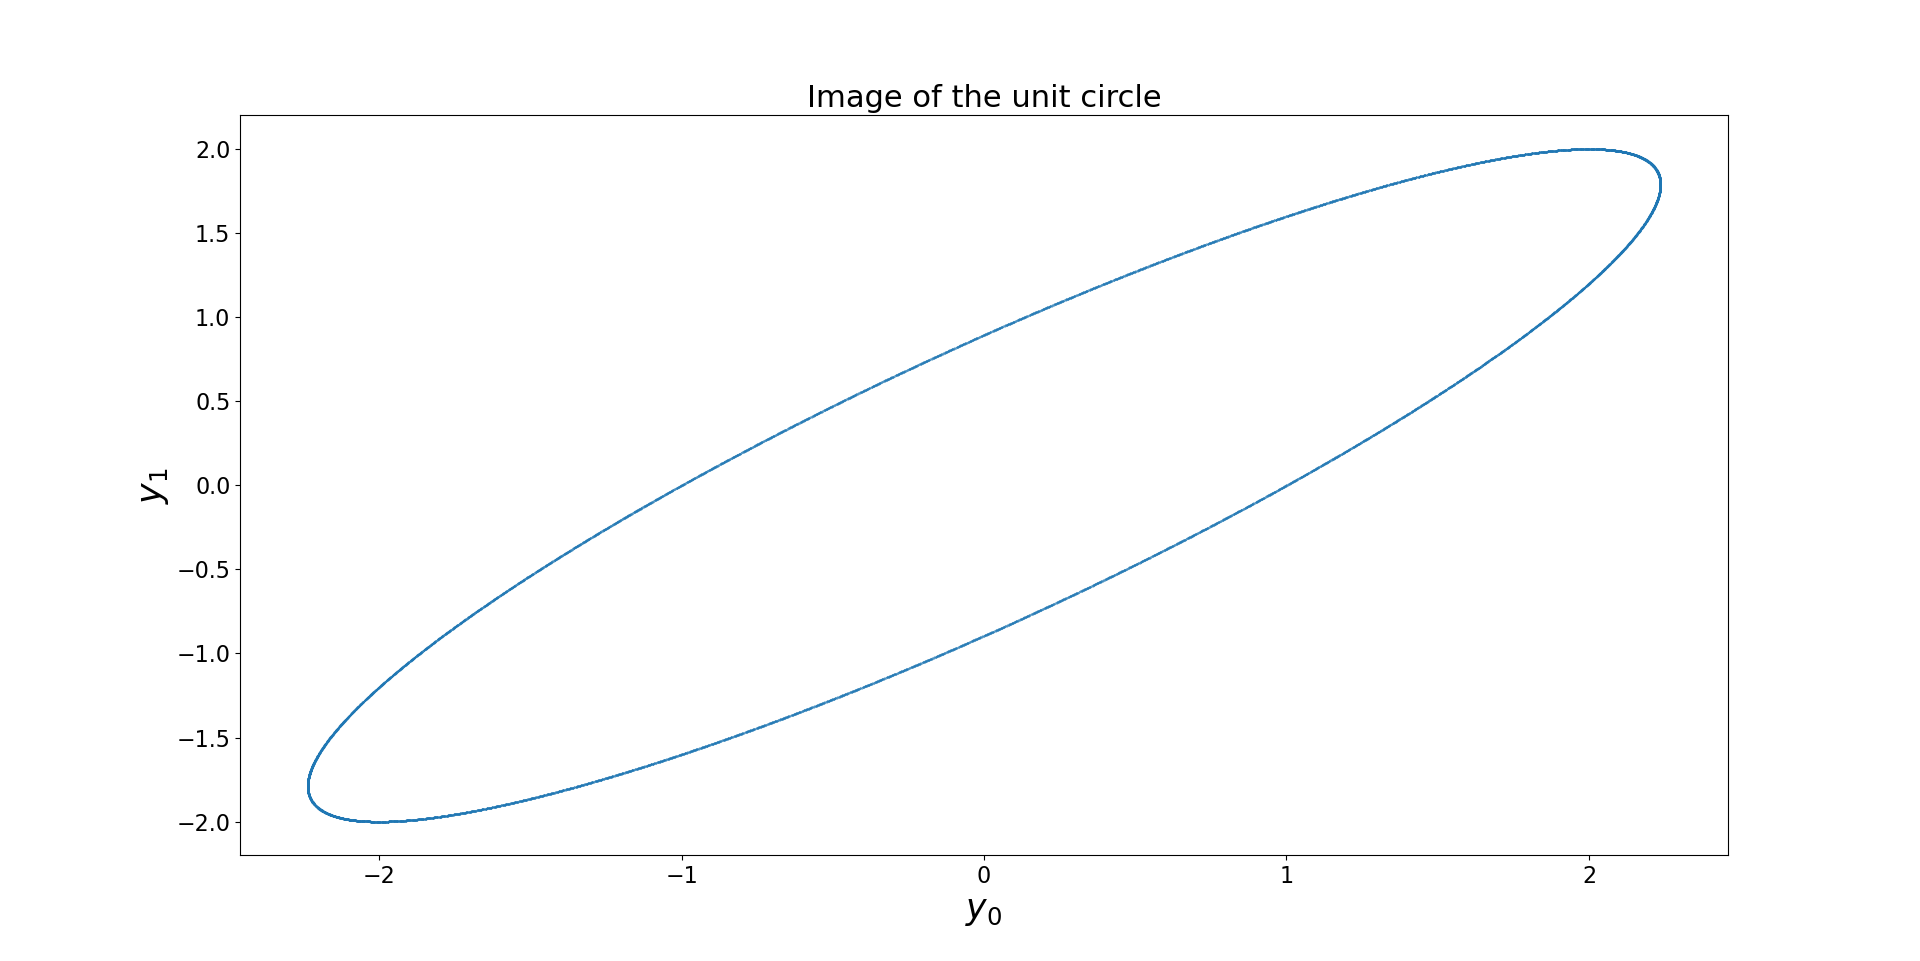
\includegraphics[scale=0.25]{Plot/Image_unit_circle}
	\caption{Image of the unit circle}
	\label{fig:Image_unit_circle}
\end{figure}

\noindent \textbf{(3)} jvejkvbkdjf\\


\noindent \textbf{(4)} Given a matrix
\begin{equation}
	A = \begin{bmatrix}
		-4 & -2 & -4 & -2 \\
		2 & -2 & 2 & 1 \\
		-800 & 200 & -800 & -401
	\end{bmatrix}.
\end{equation}
we want to compute the the singular values of $A$, the Moore-Penrose pseudoinverse of $A$ and its spectral condition number. We report in the following the Python script that we used to do it.

\begin{minted}[mathescape, linenos, breaklines]{python}
import numpy as np

A = np.array([[-4.,-2.,-4.,-2.],[2.,-2.,2.,1.],[-800,200,-800,-401]])
U, singular_values, V_transpose = np.linalg.svd(A, compute_uv=True)
pseudoinverse = np.linalg.pinv(A)
spectral_cond_num = np.linalg.cond(A)
print(f'singular values of A = {singular_values}')
print(f'pseudoinverse of A = {pseudoinverse}')
print(f'spectral condition number of A = {spectral_cond_num}')
\end{minted}

\noindent The results we obtained are reported below:

\begin{minted}{text}
singular values of A = [1.21689895e+03 3.30829410e+00 4.21538860e-03]
pseudoinverse of A = [[-2.50833333e+01  5.00833333e+01  2.50000000e-01]
		     [-1.66666667e-01 -3.33333333e-01  7.57226996e-16]
		     [-2.50833333e+01  5.00833333e+01  2.50000000e-01]
		     [ 1.00000000e+02 -2.00000000e+02 -1.00000000e+00]]
spectral condition number of A = 288680.1350686104
\end{minted}

\noindent Given the obtained results, we can say that $\text{rank}(A)=3$.\\

\noindent \textbf{(5)} The best rank-k approximation of a matrix $A$, in the Frobenius norm, is obtained by computing the singular value decomposition of $A$ and then by considering only the first $k$ terms in that expression. In other words, given a matrix $A$ written in terms of its singular value decomposition as $A = \sum_{i=1}^{n}\sigma_{i}\textbf{u}_{i}\textbf{v}_{i}^{T}$, its best rank-k approximation is given by $\tilde{A}_{k} = \sum_{i=1}^{k}\sigma_{i}\textbf{u}_{i}\textbf{v}_{i}^{T}$. Below is reported the Python code that we used to obtain the best rank-1 and rank-2 approximations of the matrix $A$ mentioned in the previous point of this exercise.

\begin{minted}[mathescape, linenos, breaklines]{python}
A_rank_1 = singular_values[0]*np.outer(U[:,0],V_transpose[0])
A_rank_2 = A_rank_1 + singular_values[1]*np.outer(U[:,1],V_transpose[1])
spectral_cond_num_A_rank_2 = singular_values[0]/singular_values[1]
print(f'A_rank_1 = {A_rank_1}')
print(f'A_rank_2 = {A_rank_2}')
print(f'Spectral condition number of A_rank_2 = {spectral_cond_num_A_rank_2}')
\end{minted}

\noindent We obtained the following two matrices:

\begin{minted}{text}
A_rank_1 = [[-3.67478811e+00  9.18652344e-01 -3.67478811e+00 -1.84198740e+00]
            [ 2.16152803e+00 -5.40355726e-01  2.16152803e+00  1.08346585e+00]
            [-8.00001057e+02  1.99990537e+02 -8.00001057e+02 -4.01000500e+02]]

A_rank_2 = [[  -3.99955481   -2.00000178   -3.99955481   -2.00177721]
            [   1.99910978   -1.99999645    1.99910978    1.00355377]
            [-800.00000445  200.00000002 -800.00000445 -400.99998223]]
            
Spectral condition number of A_rank_2 = 367.8327598758788
\end{minted}

\noindent As we can see, the best rank-1 approximation of $A$ returns a matrix that is already quite similar to the initial one, and the approximation improves when considering the best rank-2 approximation of $A$. This can be seen, in a more quantitative way, by considering the Frobenius norm of the difference between the approximated matrix and the initial matrix, both for the rank-1 and rank-2 approximation. By doing this, one obtains:

\begin{minted}{text}
Frobenious norm between A and A_rank_1 = 3.308296788282531
Frobenious norm between A and A_rank_2 = 0.004215388599497665
\end{minted}

\noindent \textbf{(6)} Consider an upper triangular matrix matrix $R = (r_{ij})$, whose entries are given by $r_{ii} = 1$ and $r_{ij} = -1$ for $j>i$. We defined a function \mintinline{python}{R_matrix(n)} that allows us to compute this matrix for a given dimension $n$:
\begin{minted}{python}
def R_matrix(n):
 R = np.triu(-np.ones((n,n)),k=1) + np.eye(n)
 return R
\end{minted}
Note that we used an upper triangular mask to obtain the entries $r_{ij}$. Once derived $R$, we computed its singular values for $n = 10,20,50,100$, as required. The plot of the singular values are reported below. 
\begin{figure}[H]
	\centering
	\subfloat[][n=10]{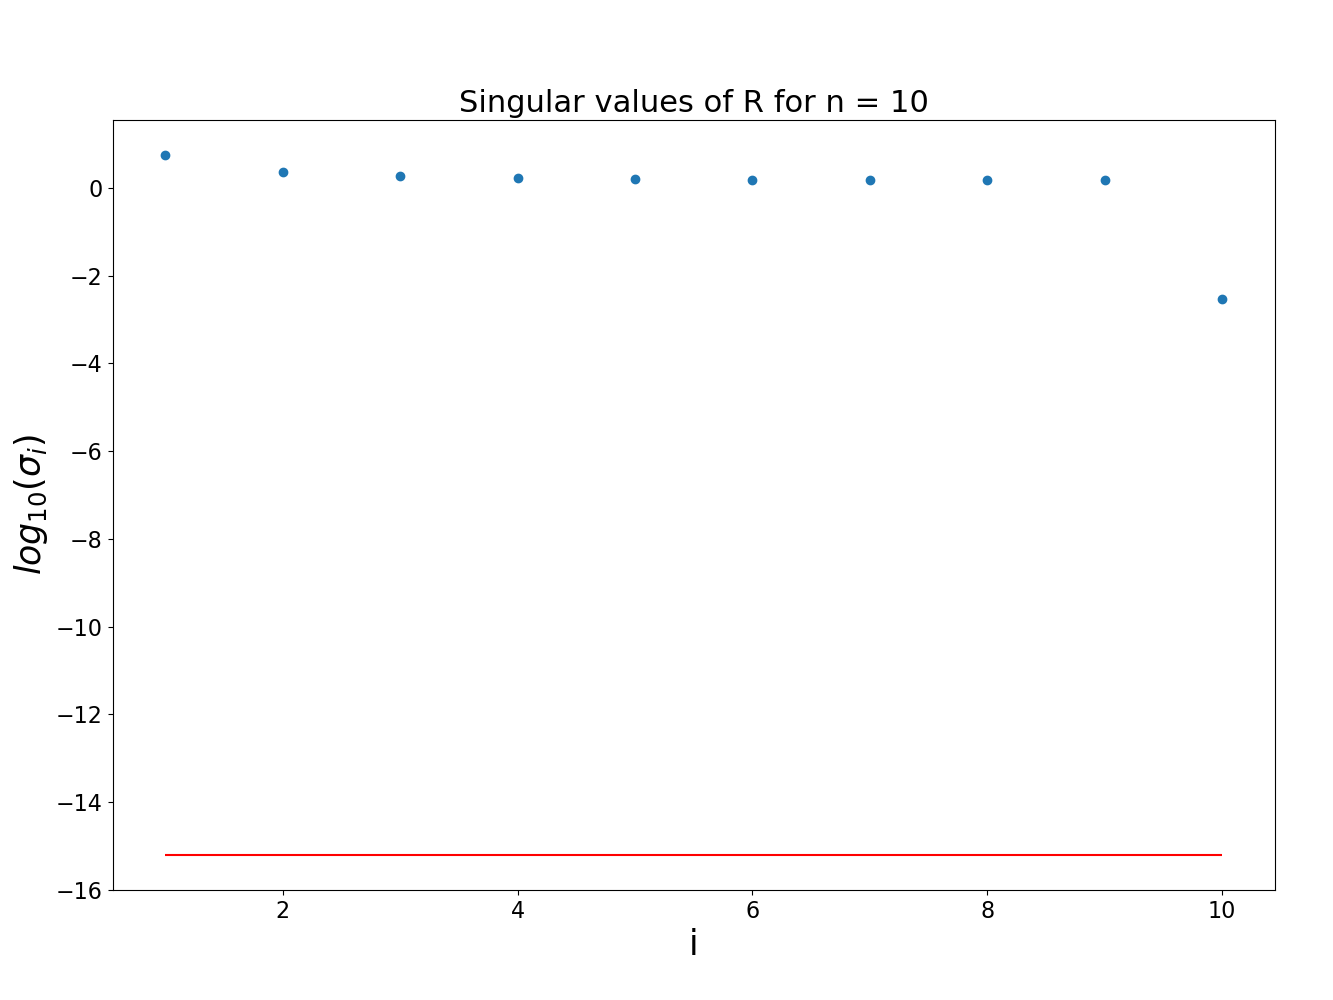
\includegraphics[scale=0.23]{Plot/Singular_values_of_R_for_n=10}} \qquad \subfloat[][n=20]{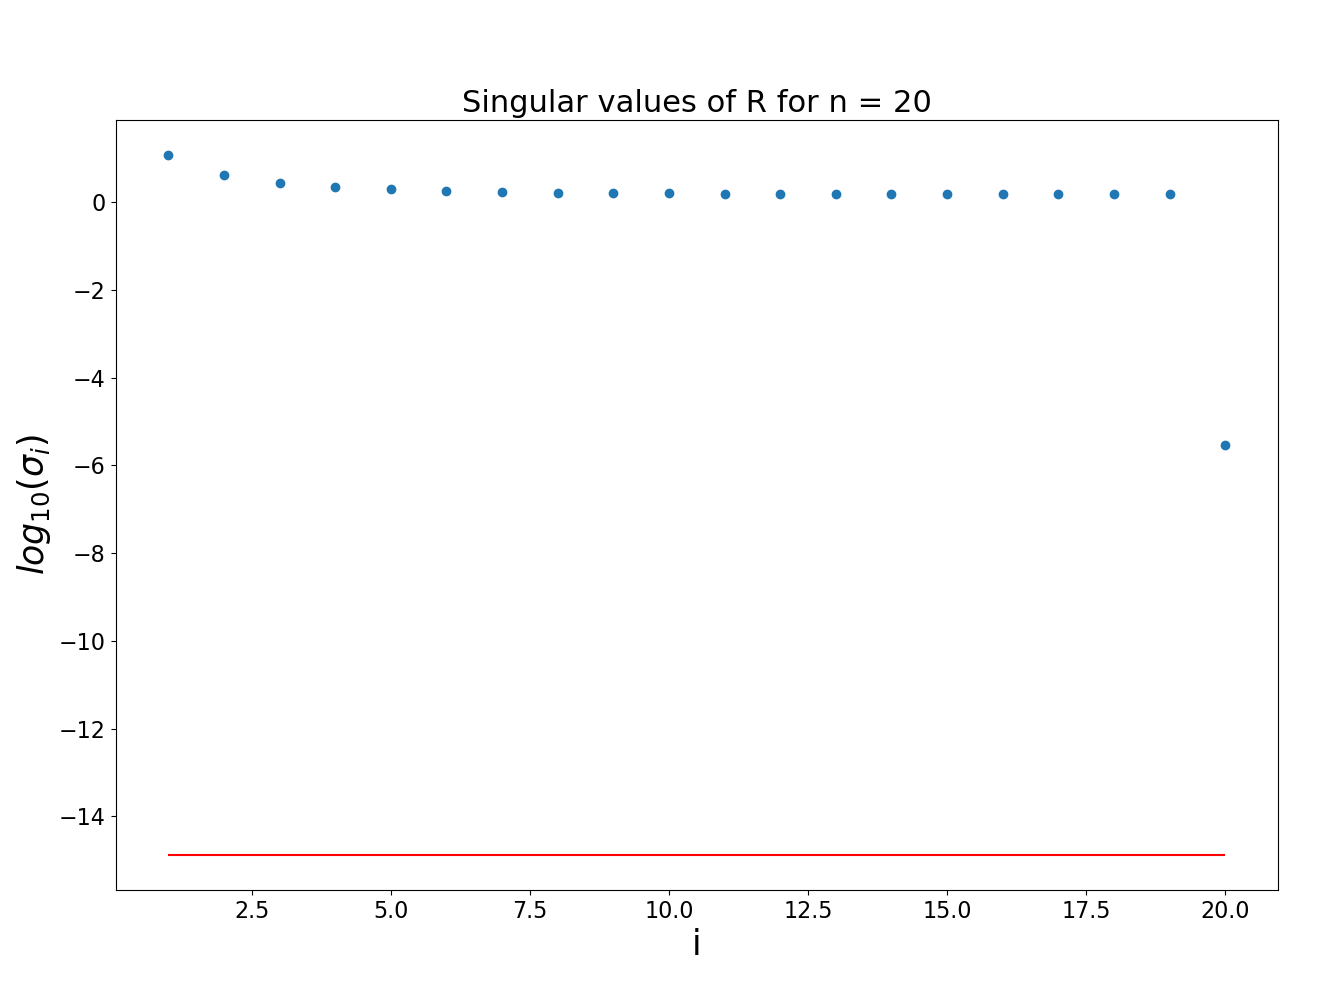
\includegraphics[scale=0.23]{Plot/Singular_values_of_R_for_n=20}} \\
	\subfloat[][n=50]{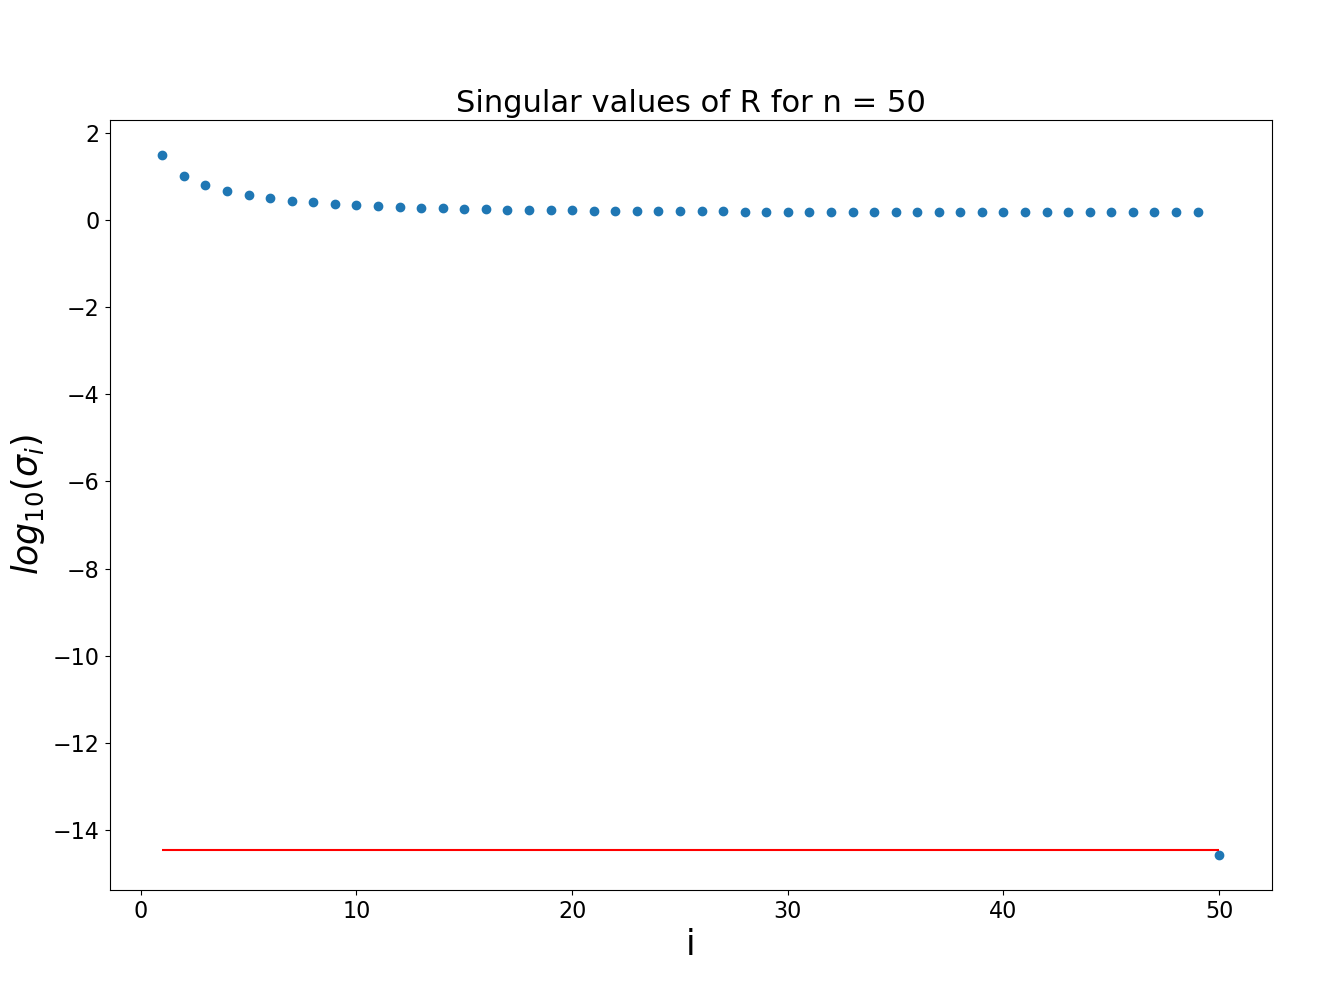
\includegraphics[scale=0.23]{Plot/Singular_values_of_R_for_n=50}} \qquad
	\subfloat[][n=100]{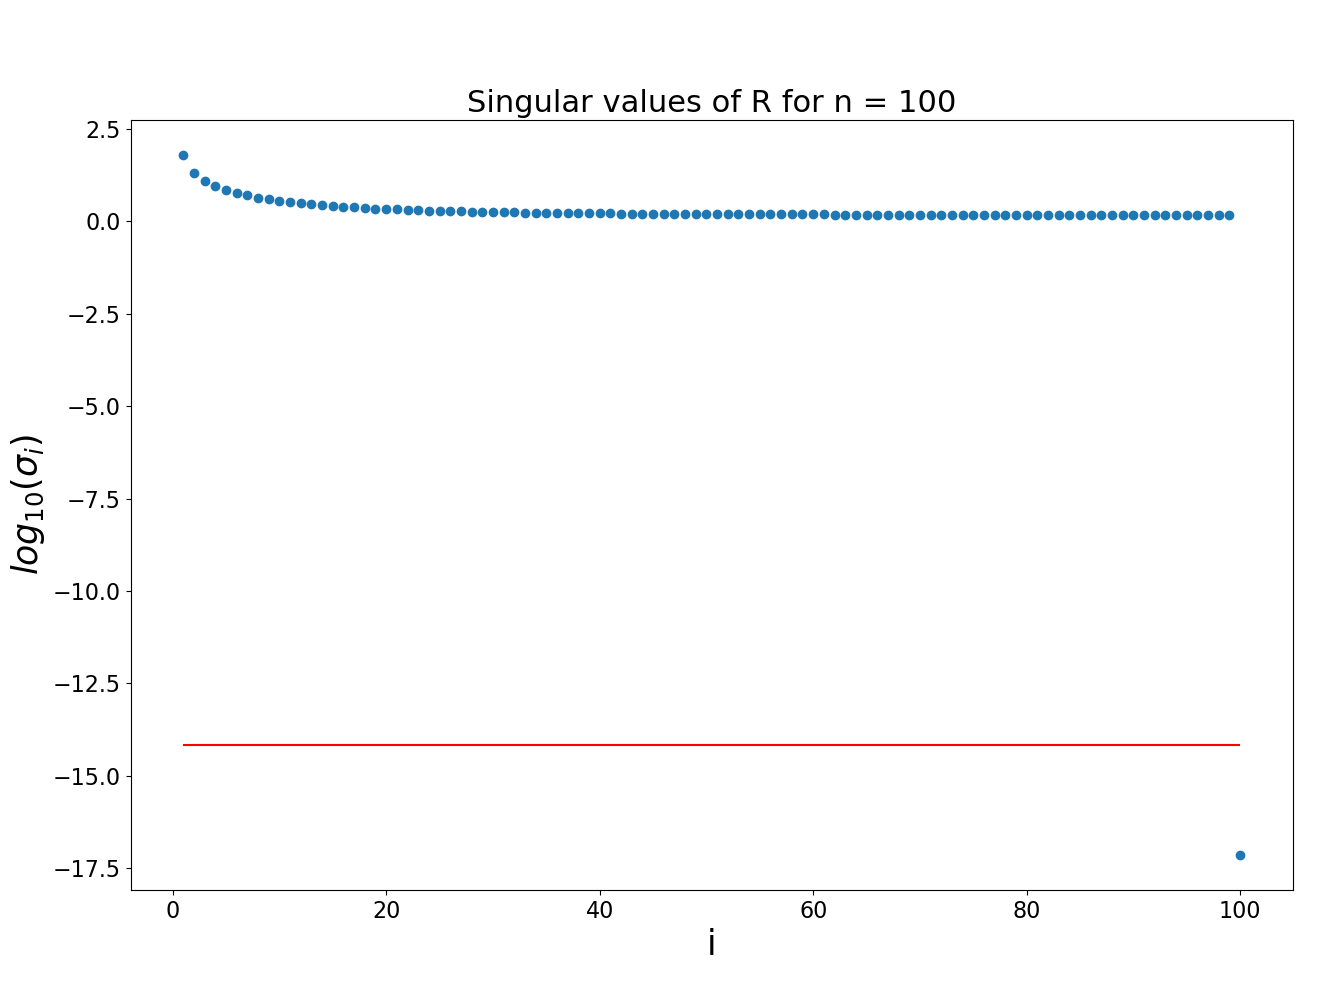
\includegraphics[scale=0.23]{Plot/Singular_values_of_R_for_n=100}}
	
	\caption{Singular values of the matrix $R$ defined at the beginning of this exercise for $n=10,20,50,100$.}
	\label{fig:Singular_values_of_R_for_different_dimensions}
\end{figure}

\noindent It can be observed that for $n=50$ and for $n=100$ the last singular value becomes smaller than the threshold value fixed by $u\sigma_{1}$, where $u$ is the machine precision. This means that, when this happens, the matrix $R$ becomes numerically singular.

\begin{figure}[H]
	\centering
	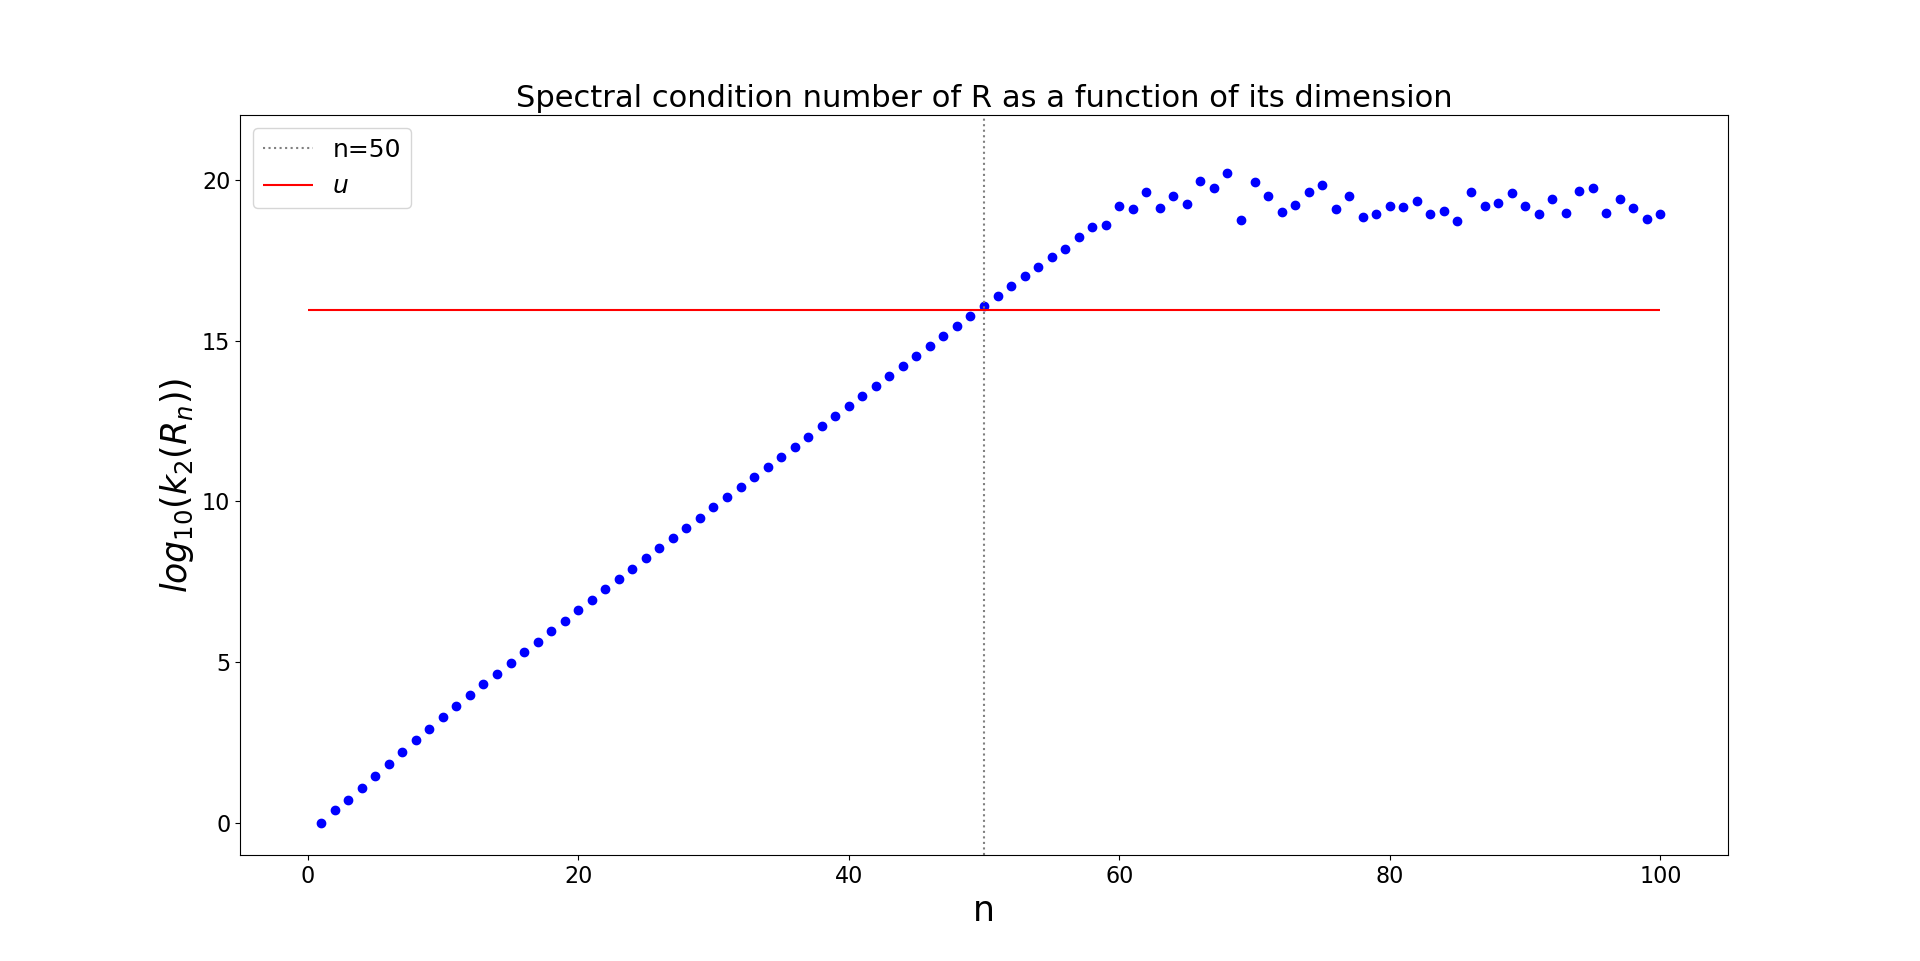
\includegraphics[scale=0.25]{Plot/Spectral_cond_num_R}
	\caption{Spectral condition number of $R$ as a function of its dimension.}
	\label{fig:Spectral_cond_num_R}
\end{figure}

\end{document}